\section{Experiments and Results}
\label{sec:exp}

\subsection{Experimental Setup}
\label{sec:exp:setup}

\paragraph{Data.}
We evaluate on three core datasets of the BOP benchmark~\cite{hodan2020bop}.
\textbf{LM-O}~\cite{brachmann2014lmo}: 8 objects, test on 200 real images with 1,445 annotated
instances (BOP19 targets), training on the PBR images of LM~\cite{hinterstoisser2012lm} (320,959 instances in scenes 0--47).
\textbf{YCB-V}~\cite{xiang2018posecnn}: 21 objects, test on 900 real images with 4,123
instances, training on 626,520 PBR instances; unlike most YCB-V entries, we do not use the real
training images. \textbf{T-LESS}~\cite{hodan2017tless}: 30 texture-less industrial objects, 27 of
them symmetric, several instances of the same object per image; test on the 1,000 Primesense images
of the BOP19 targets (6,423 instances). \pending{T-LESS training is running.}

\paragraph{Evaluation metrics.}
We report the official BOP19 average recall, $\mathrm{AR} = (\mathrm{AR}_{\mathrm{VSD}} +
\mathrm{AR}_{\mathrm{MSSD}} + \mathrm{AR}_{\mathrm{MSPD}})/3$, computed with the BOP
toolkit~\cite{hodan2020bop}. VSD measures the visible-surface discrepancy, MSSD the maximum 3D
surface distance, and MSPD the maximum 2D projection distance, each averaged over a range of
thresholds and over the symmetric poses of the object. Unless stated otherwise, we use the
default 2D detections of the BOP 2023 challenge (GDRNPP detector trained on PBR
images~\cite{liu2022gdrnpp}), which makes our numbers comparable with the leaderboard; results with
ground-truth boxes are given as an upper bound of the detector.

\paragraph{Implementation details.}
We use ViT-B/16 at $384 \times 384$ pixels with SWAG weights~\cite{singh2022swag}, the Muon
optimizer~\cite{jordan2024muon} without weight decay, a learning rate decaying from
$10^{-4}$ to $10^{-6}$ with cosine warm restarts ($T_0 = 10$ epochs, $T_\mathrm{mult} = 2$), 150
epochs and a batch size of 32. An epoch contains 21,104 instances per object (``4$\times$''
budget: 168,832 per epoch on LM-O, 443,184 on YCB-V); ablations use half of it (``2$\times$'').
The final LM-O model trains in about 34\,h on one NVIDIA A100. We report the weights of the last
epoch, which give the same AR as the best validation checkpoint (0.6685 vs.\ 0.6686 on LM-O,
0.7021 for both on YCB-V). Every ablation is trained with two random seeds.

\paragraph{Training losses.}
The total loss is the sum of the relative translation loss on $\U$ (\cref{sec:method:translation})
and the symmetry-aware rotation loss of \cref{eq:symloss}, with equal weights.

\subsection{Comparison with the State of the Art}
\label{sec:exp:sota}

\Cref{tab:lmo,tab:ycbv} compare \ours{} with the RGB entries of the BOP leaderboard that are
trained on the provided PBR images only (training data, number of models and refinement as stated
on each submission page). On YCB-V, \ours{} reaches 0.702 AR and ranks third among these methods,
behind ZebraPose and GDRNPP (0.729 and 0.713), which train one network per object, and ahead of
every other method that uses one model for all objects, including the direct methods PoseDETR
(0.679) and MRC-Net (0.681). On LM-O, it reaches 0.668: here several single-model methods are more
accurate, in particular the ViT-based direct regression PViT-6D~\cite{stapf2023pvit6d} (0.740),
the single-stage PoseDETR (0.695) and RACE-6D (0.683), and the render-and-compare methods MRPE and
RADet+PFA. \todo{Positioning to decide with the supervisor (see the note in the PR / summary):
the draft can no longer claim ``best direct-regression method''.}

Our 2D alignment (AR$_\mathrm{MSPD}$) is close to the best methods (0.873 vs.\ 0.877--0.889 on
LM-O, 0.834 vs.\ 0.821--0.831 on YCB-V, where it is the highest of the table); the gap lies in the
3D metrics (VSD and MSSD), which are dominated by the depth of the directly regressed
translation. \todo{Turn this into the ``honest weaknesses'' paragraph of the WACV paper: PBR-only,
no refinement, one network, plain ViT with a linear head, released data only, reproducible.}

\begin{table*}[t]
  \centering
  \small
  \begin{tabular}{lllcccccc}
    \toprule
    Method & Pose from & Ref. & Models & AR$\uparrow$ & AR$_\mathrm{VSD}\uparrow$ &
    AR$_\mathrm{MSSD}\uparrow$ & AR$_\mathrm{MSPD}\uparrow$ & Time [s]$\downarrow$ \\
    \midrule
    RADet+PFA~\cite{hai2023radet,hu2022pfa} & flow to renderings & Yes & one & 0.745 & 0.597 & 0.761 & 0.877 & 2.604 \\
    PViT-6D~\cite{stapf2023pvit6d} & direct regression (ViT) & No & one & 0.740 & 0.588 & 0.753 & 0.877 & 0.250 \\
    ZebraPose~\cite{su2022zebrapose} & corresp.\ + PnP & No & per object & 0.729 & 0.562 & 0.736 & 0.888 & 0.250 \\
    MRPE & render-and-compare & Yes & one & 0.715 & 0.555 & 0.701 & 0.889 & 0.097 \\
    GDRNPP~\cite{liu2022gdrnpp} & geometry-guided regr. & No & per object & 0.713 & 0.549 & 0.701 & 0.887 & 0.206 \\
    PoseDETR & direct, single stage & No & one & 0.695 & 0.543 & 0.695 & 0.847 & 0.012 \\
    MRC-Net~\cite{li2024mrcnet} & regression + residual corr. & ? & one & 0.685 & 0.523 & 0.678 & 0.853 & 1.420 \\
    RACE-6D & single stage & ? & one & 0.683 & 0.534 & 0.684 & 0.832 & 0.012 \\
    \textbf{\ours{} (Ours)} & \textbf{direct regression (ViT)} & \textbf{No} & \textbf{one} & \textbf{0.668} & 0.491 & 0.641 & 0.873 & 0.099 \\
    SurfEmb~\cite{haugaard2022surfemb} & corresp.\ + pose scoring & Yes & ? & 0.663 & 0.497 & 0.640 & 0.851 & 11.804 \\
    CosyPose~\cite{labbe2020cosypose} & render-and-compare & Yes & one & 0.633 & 0.480 & 0.606 & 0.812 & 0.550 \\
    CDPNv2~\cite{li2019cdpn} & corresp.\ + PnP & No & ? & 0.624 & 0.445 & 0.612 & 0.815 & 0.163 \\
    EPOS~\cite{hodan2020epos} & corresp.\ + PnP & No & one & 0.547 & 0.389 & 0.501 & 0.750 & 0.468 \\
    \midrule
    \ours{}, ground-truth boxes (oracle) & & & one & 0.689 & 0.514 & 0.660 & 0.892 & 0.053 \\
    \ours{}, TensorRT FP16 & & & one & 0.669 & 0.491 & 0.642 & 0.873 & \\
    \ours{}, own LW-DETR, TensorRT FP16 & & & one & 0.654 & & & & see \cref{tab:latency} \\
    \bottomrule
  \end{tabular}
  \caption{\textbf{LM-O test, RGB methods trained on the provided PBR images only}, BOP19 metrics
  (BOP leaderboard, checked 2026-11-11). ``Ref.'': iterative refinement or render-and-compare;
  ``?'': not stated on the submission page. Times per image as submitted, on each author's
  hardware (PoseDETR: RTX 4090 with TensorRT FP16; RACE-6D: RTX 3090; ours: one A100, PyTorch,
  including the 81.6\,ms of the default detector as reported by its authors). PoseDETR and RACE-6D
  include their own detection; we use the default detections of the BOP 2023 challenge.
  \todo{Entries with unknown training data (IL-Pose 0.772, ModalOcclusion-RGB 0.717) are left out;
  methods trained on real images too (HccePose, HGBPose, GPose) are not listed. Cite MRPE,
  PoseDETR and RACE-6D (CVPR 2026 Findings) once their papers are out; add our AR components for the
  own-detector row.}}
  \label{tab:lmo}
\end{table*}

\begin{table}[t]
  \centering
  \setlength{\tabcolsep}{2.5pt}
  \footnotesize
  \begin{tabular}{lcccccc}
    \toprule
    Method & Ref. & Models & AR$\uparrow$ & VSD & MSSD & MSPD \\
    \midrule
    ZebraPose~\cite{su2022zebrapose} (2023 det.) & No & per obj. & 0.729 & 0.640 & 0.725 & 0.821 \\
    GDRNPP~\cite{liu2022gdrnpp} & No & per obj. & 0.713 & 0.599 & 0.708 & 0.831 \\
    \textbf{\ours{} (Ours)} & \textbf{No} & \textbf{one} & \textbf{0.702} & 0.591 & 0.681 & \textbf{0.834} \\
    ZebraPose~\cite{su2022zebrapose} & No & per obj. & 0.691 & 0.607 & 0.686 & 0.780 \\
    MRC-Net~\cite{li2024mrcnet} & ? & one & 0.681 & 0.572 & 0.666 & 0.804 \\
    PoseDETR & No & one & 0.679 & 0.578 & 0.682 & 0.779 \\
    RADet+PFA~\cite{hai2023radet,hu2022pfa} & Yes & one & 0.648 & 0.550 & 0.623 & 0.771 \\
    SurfEmb~\cite{haugaard2022surfemb} & Yes & ? & 0.647 & 0.548 & 0.620 & 0.773 \\
    SC6D~\cite{cai2022sc6d} & ? & ? & 0.612 & 0.506 & 0.589 & 0.741 \\
    CosyPose~\cite{labbe2020cosypose} & Yes & one & 0.574 & 0.516 & 0.554 & 0.653 \\
    MRPE & Yes & one & 0.552 & 0.490 & 0.528 & 0.638 \\
    EPOS~\cite{hodan2020epos} & No & one & 0.499 & 0.411 & 0.464 & 0.621 \\
    \midrule
    Ours, GT boxes (oracle) & & one & 0.707 & & & \\
    Ours, TensorRT FP16 & & one & 0.702 & 0.591 & 0.681 & 0.834 \\
    \bottomrule
  \end{tabular}
  \caption{\textbf{YCB-V test, RGB methods trained on PBR images only} (no real training images),
  BOP19 metrics (leaderboard, checked 2026-11-11). Methods trained on the real YCB-V images reach
  up to 0.86 (\eg PViT-6D 0.832, RACE-6D 0.782). ``Ref.'': refinement; ``?'': not stated.
  \todo{Check SC6D and SurfEmb details; add times.}}
  \label{tab:ycbv}
\end{table}

\paragraph{T-LESS.}
\pending{T-LESS results (\texttt{tless-m10-tok4x\{,2\}}, running): AR with default detections and
with GT boxes, comparison table as for LM-O and YCB-V.}

\subsection{Ablation Studies}
\label{sec:exp:ablations}
All ablations are evaluated with the official AR on LM-O test with the default detections. Unless
stated otherwise, each experiment changes one component of the ablation baseline: our final
configuration at the 2$\times$ budget (AR 0.655 for both seeds). We report both seeds; the seed
spread is typically 0.002--0.008 AR, so smaller differences are not significant.

\paragraph{Translation and rotation targets.}
\Cref{tab:abl_targets} validates the two geometric choices. Regressing the absolute rotation
instead of the apparent one costs 0.108 AR, and every object loses (the eggbox the most, from
0.32 to 0.18): the main finding of~\cite{ancey2026fastposevit} holds in the multi-object setting.
The original depth target costs 0.038 AR; the loss is largest for the large objects (driller
0.79 $\rightarrow$ 0.70, can 0.80 $\rightarrow$ 0.75), as expected from a target that scales with
the object size. On the driller alone, the gap was already 0.06 AR (0.844 vs.\ 0.785, single-object
models).

\begin{table}[t]
  \centering
  \small
  \begin{tabular}{llcc}
    \toprule
    Component & Choice & AR (seed a / b)$\uparrow$ & Mean \\
    \midrule
    \multirow{2}{*}{Rotation target} & \textbf{apparent} & \textbf{0.655 / 0.655} & \textbf{0.655} \\
     & absolute & 0.546 / 0.548 & 0.547 \\
    \midrule
    \multirow{2}{*}{Depth target} & \textbf{site, \cref{eq:uz}} & \textbf{0.655 / 0.655} & \textbf{0.655} \\
     & legacy~\cite{ancey2026fastposevit} & 0.610 / 0.625 & 0.617 \\
    \midrule
    \multirow{2}{*}{Pre-training} & \textbf{SWAG} & \textbf{0.655 / 0.655} & \textbf{0.655} \\
     & none (scratch) & 0.516 / 0.517 & 0.517 \\
    \bottomrule
  \end{tabular}
  \caption{\textbf{Targets and pre-training}, LM-O test AR with default detections, ablation
  baseline (2$\times$ budget, bold).}
  \label{tab:abl_targets}
\end{table}

\paragraph{Pre-training.}
Training from a random initialization with the same budget loses 0.138 AR
(\cref{tab:abl_targets}), on all objects: as for spacecraft~\cite{ancey2026fastposevit},
large-scale pre-training is essential when only synthetic images are available.

\paragraph{One network for all objects.}
\Cref{tab:abl_objects} compares the ways to share the network. The class token is slightly better
than per-object heads (+0.005) and combining both brings another 0.005, both at about the seed
spread; we keep the class token alone, which needs no per-object output layer. Eight
single-object models, trained with the same total compute, reach 0.672 AR, the same as the shared
model (0.668), with eight times as many parameters and no batching across objects.

\begin{table}[t]
  \centering
  \small
  \begin{tabular}{lcc}
    \toprule
    Conditioning (2$\times$) & AR (seed a / b)$\uparrow$ & Mean \\
    \midrule
    per-object heads & 0.650 / 0.650 & 0.650 \\
    \textbf{per-object class token} & \textbf{0.659 / 0.651} & \textbf{0.655} \\
    heads + class token & 0.660 / 0.661 & 0.660 \\
    \midrule
    Final model (token, 4$\times$) & 0.669 / 0.664 & 0.666 \\
    8 single-object models (4$\times$ total) & 0.672 (1 seed) & \\
    \bottomrule
  \end{tabular}
  \caption{\textbf{Sharing one network across the 8 LM-O objects}, LM-O test AR with default
  detections.}
  \label{tab:abl_objects}
\end{table}

\paragraph{Training compute.}
\Cref{tab:abl_budget} varies the number of samples per epoch at a fixed number of epochs. More
compute helps on both datasets: on LM-O, AR rises from 0.639 to 0.661 between the 1$\times$ and
4$\times$ budgets (per-object heads); on YCB-V, with 21 objects, 4$\times$ beats 2$\times$ by
0.013 AR, and both 4$\times$ seeds are above both 2$\times$ seeds. We use 4$\times$ for the final
models and 2$\times$ for the ablations.

\begin{table}[t]
  \centering
  \small
  \begin{tabular}{llccc}
    \toprule
    Dataset & Conditioning & 1$\times$ & 2$\times$ & 4$\times$ \\
    \midrule
    LM-O & heads & 0.641 / 0.637 & 0.650 / 0.650 & 0.661 \\
    LM-O & token & & 0.659 / 0.651 & 0.669 / 0.664 \\
    YCB-V & token & & 0.681 / 0.689 & 0.694 / 0.702 \\
    \bottomrule
  \end{tabular}
  \caption{\textbf{Training budget}, test AR with default detections (seed a / b). 1$\times$ =
  5,276 samples per object and epoch, 150 epochs. The final YCB-V model (0.702) was selected on
  the PBR validation split.}
  \label{tab:abl_budget}
\end{table}

\paragraph{Components without a measurable effect.}
Several choices did not change the test AR beyond the seed spread: the choice between the
``domain gap'' augmentation and a standard photometric set (0.639 vs.\ 0.637; using no
augmentation at all does hurt, \cref{tab:abl_aug}), the symmetry-aware loss (0.655
both; it is needed for symmetries with offsets on YCB-V, \cref{sec:method:symmetry}), the training
crop (visible box 0.655, amodal box 0.648, random mix 0.652), and a decoupled translation loss. We
report them for completeness. \todo{Decide which of these go to the supplementary material.}

\paragraph{Bounding-box perturbation.}
\Cref{tab:abl_bbox} shows that perturbing the training boxes is important: without it, the AR drops
by 0.030. Perturbations of 10\,\% and 20\,\% per side give the same AR.
\pending{5\,\%, 15\,\% and 30\,\% (jobs queued).}

\begin{table}[t]
  \centering
  \small
  \begin{tabular}{lcc}
    \toprule
    Perturbation per side & AR (seed a / b)$\uparrow$ & Mean \\
    \midrule
    0\,\% & 0.625 / 0.625 & 0.625 \\
    5\,\% & \pending{} & \\
    \textbf{10\,\%} & \textbf{0.655 / 0.655} & \textbf{0.655} \\
    15\,\% & \pending{} & \\
    20\,\% & 0.650 / 0.651 & 0.650 \\
    30\,\% & \pending{} & \\
    \bottomrule
  \end{tabular}
  \caption{\textbf{Bounding-box perturbation during training}, LM-O test AR with default
  detections, ablation baseline.}
  \label{tab:abl_bbox}
\end{table}

\paragraph{Pixel augmentations.}
\label{sec:exp:augmentations}
Photometric augmentation is needed to cross the gap from PBR training images to real test
images: without it, the AR drops by 0.028 (\cref{tab:abl_aug}), with the largest losses on the
glue (0.67 $\rightarrow$ 0.53) and the can (0.80 $\rightarrow$ 0.75). Which operations matter
is less clear: the ``domain gap'' set and a standard photometric set give the same AR (0.639 vs.\
0.637 with per-object heads, 1$\times$). \pending{Color, blur and noise alone, their
combination, and ``domain gap'' with $p = 0.8$ (jobs running).}

\begin{table}[t]
  \centering
  \small
  \begin{tabular}{lcc}
    \toprule
    Pixel augmentation & AR (seed a / b)$\uparrow$ & Mean \\
    \midrule
    none & 0.626 / 0.629 & 0.628 \\
    color only & \pending{} & \\
    blur only & \pending{} & \\
    noise only & \pending{} & \\
    color + blur + noise & \pending{} & \\
    \textbf{domain gap ($p = 0.5$)} & \textbf{0.655 / 0.655} & \textbf{0.655} \\
    domain gap ($p = 0.8$) & \pending{} & \\
    \bottomrule
  \end{tabular}
  \caption{\textbf{Pixel augmentations}, LM-O test AR with default detections, ablation
  baseline. Each operation is applied independently with probability $p$.}
  \label{tab:abl_aug}
\end{table}

\paragraph{Detection quality.}
With ground-truth boxes, the AR rises from 0.668 to 0.689 on LM-O and from 0.702 to 0.707 on
YCB-V: the detector accounts for a small part of the remaining error. On LM-O, the eggbox, our
weakest object (0.36 AR), also has the worst detections: 27\,\% of its default boxes overlap the
ground truth by less than 0.5 IoU (6.3\,\% over all objects). Per-object results are in
\cref{sec:appendix:perobject}.

\subsection{Model Compression and Deployment}
\label{sec:exp:deployment}

\paragraph{Export.}
We export the network to ONNX with a dynamic batch dimension (one crop per detected object, plus
the object index of each crop) and build a TensorRT engine with one optimization profile for 1 to
16 crops. The ONNX outputs match PyTorch to $3 \cdot 10^{-6}$, and the FP16 engine changes the AR
by at most 0.0004 (LM-O 0.6685 for both, YCB-V 0.7017 vs.\ 0.7021). \Cref{tab:size} gives the size
of the network: sharing it across objects costs fewer than 0.05\,M parameters.

\begin{table}[t]
  \centering
  \small
  \begin{tabular}{lccc}
    \toprule
    Input & Objects & Params [M] & GFLOPs / crop \\
    \midrule
    224 px & 8 / 21 & 85.81 / 85.82 & 17.6 \\
    384 px & 8 / 21 & 86.10 / 86.11 & 55.5 \\
    \bottomrule
  \end{tabular}
  \caption{\textbf{Network size}, with per-object class tokens. GFLOPs counted as multiply-adds,
  as in~\cite{ancey2026fastposevit}. TensorRT FP16 engine: 167\,MB.}
  \label{tab:size}
\end{table}

\paragraph{Latency.}
\Cref{tab:latency} reports the latency per image as a function of the number of objects $N$, on one
NVIDIA A100 (CUDA 13, TensorRT 10.14, PyTorch 2.9). The \emph{pipeline} time starts from the decoded
image and the boxes and ends with the $N$ absolute poses: crop and normalize every instance, run
the network once on all crops, and recover $\R$ and $\T$. Two engineering changes made the pipeline
2--3 times faster than a direct port of the single-object code: normalizing the crops on the GPU
instead of with Albumentations on the CPU (2.1\,ms per crop), and recovering the poses on the CPU
in one vectorized step instead of many small GPU operations. With TensorRT FP16, the pose stage
processes 8 objects in 14.2\,ms (70 FPS), and the latency grows linearly with $N$
(\cref{fig:latency}).

\begin{table}[t]
  \centering
  \setlength{\tabcolsep}{4pt}
  \small
  \begin{tabular}{lcccc}
    \toprule
    ms per image & $N{=}1$ & $N{=}4$ & $N{=}8$ & $N{=}16$ \\
    \midrule
    Network, PyTorch FP16 & 7.2 & 7.6 & 8.7 & 15.9 \\
    Network, TensorRT FP16 & \textbf{1.8} & \textbf{3.5} & \textbf{5.7} & \textbf{11.0} \\
    Pipeline, PyTorch FP16 & 10.8 & 13.5 & 17.0 & 29.5 \\
    Pipeline, TensorRT FP16 & \textbf{5.3} & \textbf{9.3} & \textbf{14.2} & \textbf{24.0} \\
    Pipeline, TensorRT FP16, 224 px & 4.3 & 5.8 & 7.1 & 10.6 \\
    \midrule
    + default detector (81.6\,ms) [FPS] & 11.5 & 11.0 & 10.4 & 9.5 \\
    + our LW-DETR (4.2\,ms) [FPS] & 105 & 74 & 55 & 35 \\
    + our LW-DETR, 224 px [FPS] & 118 & 100 & 88 & 68 \\
    \bottomrule
  \end{tabular}
  \caption{\textbf{Latency per image vs.\ number of objects $N$} on one NVIDIA A100 (median of
  200 runs, LM-O model, 384 px unless stated). Network: the $N$ crops already on the GPU. Pipeline:
  decoded image to $N$ poses. Default detector time as reported by its authors; our detector:
  mean time per image of its TensorRT FP16 engine over the LM-O test images (median 3.3\,ms),
  measured on the same GPU and added to the pipeline time, since both run one after the other.}
  \label{tab:latency}
\end{table}

\begin{figure}[t]
  \centering
  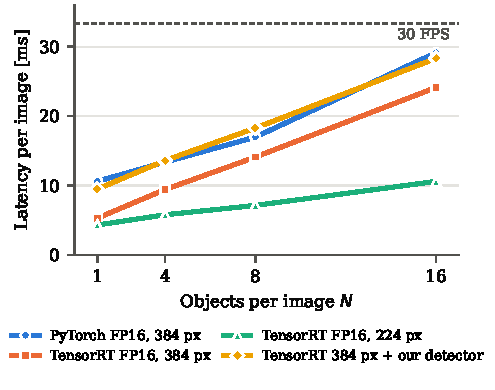
\includegraphics[width=\linewidth]{figures/latency.pdf}
  \caption{\textbf{Latency per image vs.\ number of objects} (pose pipeline from the decoded
  image to $N$ poses; LM-O model, one A100). With TensorRT FP16 and our detector, the full
  method stays above 30 FPS up to 16 objects.}
  \label{fig:latency}
\end{figure}

\paragraph{Detector.}
With the default detector (about 80\,ms per image as reported by its authors), the detector
dominates the run time and the whole method runs at about 10 FPS. Our multi-class LW-DETR
(\cref{sec:method:detector}) reaches a COCO mAP of 0.656 on the LM-O test targets, on par with
the default detections (0.657), and gives 0.654 AR with our pose model (0.645--0.650 with the
smaller ``tiny'' variant). Exporting it to TensorRT required one change: TensorRT 10.14's
\texttt{GridSample} returns wrong values for the deformable attention of LW-DETR (mAP 0.633 even
in FP32), so we implement the bilinear sampling with gather operations, which gives the same
output as PyTorch. The FP16 engine runs in 4.2\,ms per image on average (median 3.3\,ms,
including resizing, normalization and top-$k$ selection) with the same mAP (0.657), and the full
pipeline reaches 55 FPS for 8 objects at 384 px (0.654 AR), or 88 FPS at 224 px, where the
backbone costs 0.023 AR (0.643 vs.\ 0.666, two seeds each).
\todo{Jetson Orin numbers, if a device becomes available; otherwise state it as a limitation.}

\subsection{Qualitative Results}
\label{sec:exp:qualitative}
\begin{figure*}[t]
  \centering
  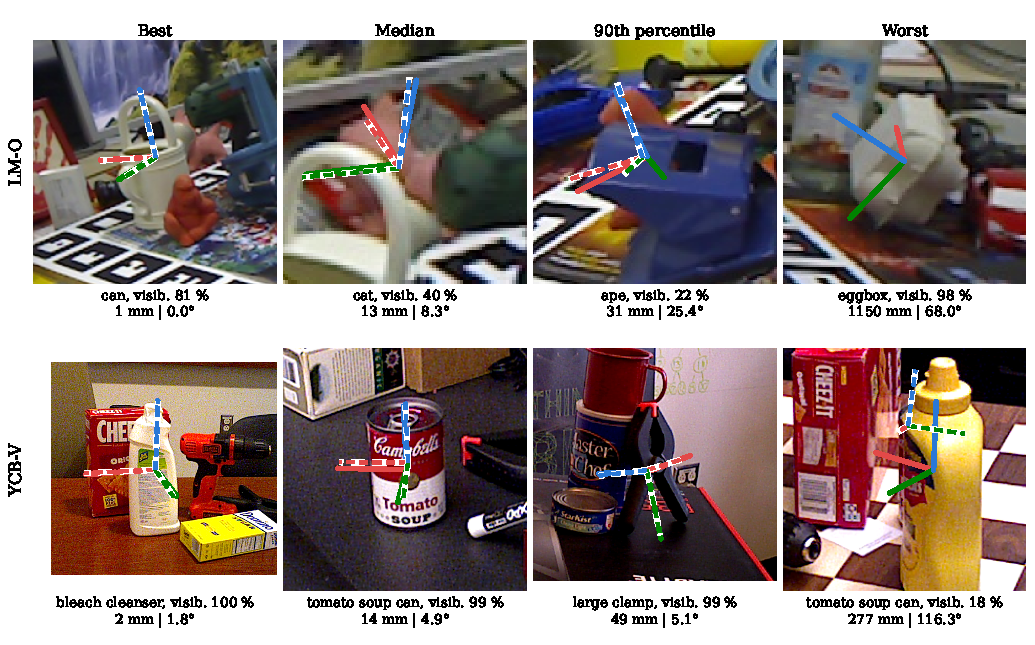
\includegraphics[width=\linewidth]{figures/qualitative.pdf}
  \caption{\textbf{Qualitative results} on LM-O (top) and YCB-V (bottom) with the default
  detections: the best, median, 90th-percentile and worst test instance, ranked by the MSSD error
  relative to the object diameter. Ground-truth axes are solid (for symmetric objects, under the
  symmetry closest to the prediction), predictions dashed; below each crop, the object, its
  visible fraction, and the translation [mm] and rotation [deg] errors. The worst LM-O case is a
  wrong detection: the predicted pose lies outside the crop.}
  \label{fig:qualitative}
\end{figure*}

\begin{figure}[t]
  \centering
  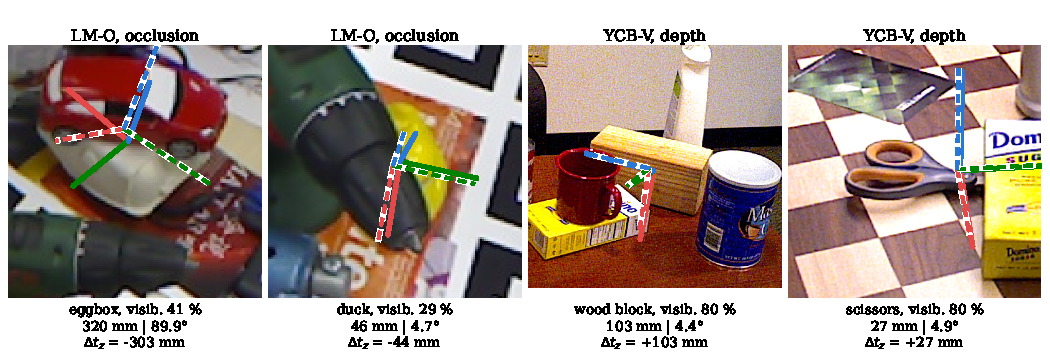
\includegraphics[width=\linewidth]{figures/failures.pdf}
  \caption{\textbf{Failure cases.} Left: heavily occluded LM-O objects (eggbox, duck), where the
  regressed depth and, for the eggbox, the rotation fail. Right: the depth bias on real YCB-V
  images; the rotation is accurate ($< 5^\circ$) but the object is estimated too far
  ($\Delta t_z > 0$).}
  \label{fig:failures}
\end{figure}

\Cref{fig:qualitative} shows typical predictions. The median errors over all test instances are
19\,mm and 4.3\textdegree{} on LM-O, and 22\,mm and 3.8\textdegree{} on YCB-V: the rotation is
usually accurate, and most of the error lies in the depth. \Cref{fig:failures} shows the two main
failure modes. First, heavily occluded objects: with less than half of the eggbox or the duck
visible, the crop contains too little of the object to regress its depth, and the eggbox, whose
appearance is ambiguous, also gets a wrong rotation. Second, a systematic depth bias on the real
YCB-V images: 89\,\% of the YCB-V instances are estimated too far (median +20\,mm), against 48\,\%
on LM-O (median $-1$\,mm). The real objects appear smaller in the images than their PBR renders
at the same depth, so a network trained on PBR images only overestimates their depth; the
weakest YCB-V objects (wood block 0.39 AR, scissors 0.41) are the most affected. Training with
the real YCB-V images should remove this bias, as it does for the methods trained on them.
